
\documentclass[12pt]{article}

\usepackage{sbc-template}
\usepackage{graphicx,url}
\usepackage[spanish]{babel}
\usepackage[utf8]{inputenc}
\usepackage{verbatim}
\usepackage{listings}
\usepackage{xcolor}
\usepackage{mips}
\usepackage{color}
\usepackage{float}
\usepackage{tikz}

\lstset{ %
  language=[mips]Assembler,       % the language of the code
  basicstyle=\footnotesize,       % the size of the fonts that are used for the code
  numbers=left,                   % where to put the line-numbers
  numberstyle=\tiny\color{gray},  % the style that is used for the line-numbers
  stepnumber=1,                   % the step between two line-numbers. If it's 1, each line
                                  % will be numbered
  numbersep=5pt,                  % how far the line-numbers are from the code
  backgroundcolor=\color{white},  % choose the background color. You must add \usepackage{color}
  showspaces=false,               % show spaces adding particular underscores
  showstringspaces=false,         % underline spaces within strings
  showtabs=false,                 % show tabs within strings adding particular underscores
  frame=single,                   % adds a frame around the code
  rulecolor=\color{black},
  tabsize=4,                      % sets default tabsize to 2 spaces
  captionpos=b,                   % sets the caption-position to bottom
  breaklines=true,                % sets automatic line breaking
  breakatwhitespace=false,        % sets if automatic breaks should only happen at whitespace
  title=\lstname,                 % show the filename of files included with \lstinputlisting;
                                  % also try caption instead of title
  keywordstyle=\color{blue},          % keyword style
  commentstyle=\color{dkgreen},       % comment style
  stringstyle=\color{mauve},         % string literal style
  escapeinside={\%*}{*)},            % if you want to add a comment within your code
  morekeywords={*,...}               % if you want to add more keywords to the set
}

\definecolor{verde}{rgb}{0,0.5,0}
\definecolor{dkgreen}{rgb}{0,0.6,0}
\definecolor{gray}{rgb}{0.5,0.5,0.5}
\definecolor{mauve}{rgb}{0.58,0,0.82}

\lstset{language=verilog,
                belowcaptionskip=1\baselineskip,
                breaklines=true,
                frame=false,
                xleftmargin=\parindent,
                showstringspaces=false,
                basicstyle=\footnotesize\ttfamily,
                keywordstyle=\bfseries\color{green!40!black},
                commentstyle=\itshape\color{purple!40!black},
                identifierstyle=\color{blue},
                stringstyle=\color{orange},
                numbers=left,
            }

\sloppy

\title{Implementación procesador MIPS\\ Facultad de Ciencias Exactas, Físicas y Naturales}

\author{Sardoy, Juan Manuel\inst{1}, Perez, Federico\inst{1}}


\address{Arquitectura de computadoras - FCEFyN\\
  Av. Velez Sarsfield 1600 --  Córdoba -- Argentina
  \email{jmsardoy@gmail.com, 0xfede07c8@gmail.com}
}

\begin{document}

\maketitle

\begin{resumen}
  Este documento describe, de manera sintética, la implementación práctica del pipeline de un procesador que cumple con un subconjunto del set de instrucciones de la arquitectura MIPS IV de 32 bits. La implementación está basada en tecnologia FPGA, mediante el lenguaje Verilog. Este trabajo tiene como objeto el aprendizaje de los diferentes elementos más comunes de la arquitectura de computadoras, dado el encuadre académico del mismo.\\
  \textbf{Palabras clave}: MIPS, FPGA, pipeline.
\end{resumen}

\begin{abstract}
  This document describes, in a synthetic way, a practical implementation of the pipeline of a processor that is compliant with a subset of the MIPS IV 32bits architecture instruction set. This job has as objective, to build the basic knowledge of the computer's architecture cope of study. \\
  \textbf{Keywords}: MIPS, FPGA, pipeline.
\end{abstract}

\section{Introducción}

El trabajo, se encuentra dentro del marco de la asignatura de Arquitectura de Computadoras, de la FCEFyN de la Universidad Nacional de Córdoba, Argentina. Corresponde al trabajo final de la misma, el cual es requerimiento para su aprobación.

Además de la implementación del procesador en sí, se mostrará como implementar los elementos auxiliares requeridos para su funcionamiento y programación, entre otras utilidades. El hardware utilizado será un dispositivo FPGA, de la marca Xilinx, al ser de esta empresa, con los que cuentan los autores del trabajo.

Dentro de los elementos auxiliares, encontraremos el desarrollo de un sistema de comunicación directo con el procesador, mediante el protocolo UART. Además de este, un mecanismo para cargar un programa en la RAM del procesador, como asi también funcionalidad de debugging (ejecución paso a paso y salída de valores de registros internos). También se mostrará la implementación y uso de software auxiliar para el ensamblado de los programas a ejecutar.

Todo esto compondrá una suite básica de desarrollo de software de propósito general, cuyo entendimiento es el objetivo principal del trabajo y la materia.


\section{Referencias Teóricas} \label{sec:firstpage}

La técnica de \textit{pipeline} es la más común utilizada para la implementación de procesadores modernos de diferentes arquitecturas, dado el gran aumento de \textit{IPC} (instrucciones por ciclo) que este provee.

MIPS son las siglas de \textit{Microprocessor without interlocked pipeline stages}. Es una arquitectura RISC (\textit{reduced instruction set computer} desarrollada por MIPS Computer Systems. Existen versiones de 32 y 64 bits de dicha arquitectura. La primera versión de fue desarrollada en la Universidad de Stanford en 1981 por un equipo liderado por John. L. Hennesy. La idea era diseñar un procesador segmentado (idea ya muy conocida en esos momentos) pero sin interbloqueo entre capas. En esa época eran comunes los procesadores donde cada instrucción iba ejecutandose por cada capaz, mientras las otras permanecian inactivas. Esto llevaba a que el tiempo que demora en ejecutar la instrucción fuera el del tiempo en el que tarda en pasar por todas las capas, en contraste con el tiempo del camino crítico, como ocurre sin interbloqueo.

Por estos motivos este trabajo tendrá como cuerpo principal, la aplicación de dicha técnica, para lo cual, a modo de guía, se seguirá la bibliografía de \textit{Patterson y Hennesy}, dado que expone y soluciona los problemas más comunes a la hora de la creación de un \textit{pipeline} genérico. Sin embargo, muchas partes de la implementación, quedan a cargo, y serán solucionadas por los autores, lo cual lo hace una implementación única de la arquitectura.

\section{Metodología}

Se utilizará una metodología incremental y modular para la implementación del pipeline y sus módulos complementarios. Esto mejora el entendimiento y fragmentación del problema, asi como también facilta su implementación, dado la complejidad del mismo. También esto es muy util a la hora del testing y el debugeado del sistema.

\section{Requerimientos del trabajo}\label{sec:consigna}

Los requerimientos provistos por la cátedra fueron los siguientes:

\begin{enumerate}
  \item Implementar el pipeline de un procesador MIPS, segmentado en las siguientes etapas:
  \begin{enumerate}
    \item \textbf{IF} (Instruction Fetch): Búsqueda de la instrucción en la memoria de programa.
    \item \textbf{ID} (Instruction Decode): Decodificación de la instrucción y lectura de registros.
    \item \textbf{EX} (Excecute): Ejecución de la instrucción propiamente dicha.
    \item \textbf{MEM} (Memory Access): Lectura o escritura desde/hacia la memoria de datos.
    \item \textbf{WB} (Write back): Escritura de resultados en los registros.
  \end{enumerate}
  \item En dicha arquitectura, implementar las siguientes instrucciones:
  \begin{enumerate}
    \item \textbf{R-type} (SLL, SRL, SRA, SLLV, SRLV, SRAV, ADDU, SUBU, AND, OR, XOR, NOR, SLT?
    \item \textbf{I-Type} (LB, LH, LW, LWU, LBU, LHU, SB, SH, SW, ADDI, ANDI, ORI, XORI, LUI, SLTI, BEQ, BNE, J, JAL)
    \item \textbf{J-Type} (JR, JALR)
  \end{enumerate}
  \item Debe poseer soporte (detección y manejo) de los siguientes tipos de riesgos:
  \begin{enumerate}
    \item \textbf{Estructurales}: Cuando dos o más instrucciones tratan de utilizar el mismo recurso en el mismo ciclo.
    \item \textbf{Datos}: Una etapa desea utilizar un dato antes de que esté listo. Se debe mantener el orden estricto de las lecturas y escrituras.
    \item \textbf{Control}: Capacidad para tomar una decición sobre una condicion no evaluada. \\
    Para esto debe implementar:
    \item \textbf{Unidad de detección} riesgos: Detecta los posibles riesgos de cada tipo, y efectua los controles necesarios.
    \item \textbf{Unidad de cortocircuitos}: Ayuda en el transpaso de datos de una etapa a otra, de ser requeridos inmediatamente. Elimina la necesidad de que los datos lleguen a la última etapa de escritura de registros para que estos sean usados por otros.
  \end{enumerate}
      \item \textbf{Ensablador:} Debe implementarse un programa ensamblador, en el cual dado una entrada en assembler de MIPS, se obtenga una salida de código máquina, apto para ser ejecutado.
      \item \textbf{Unidad de Debug:} Administra y monitorea la ejecución del procesador mediante una interfaz UART. Debe ser capaz de cargar un programa en memoria, correrlo en varios modos, y mostrar el estado del procesador. \\ \\
      \textit{Los datos que se deben envíar son:} \\
      \begin{enumerate}
        \item Contenido de los 32 registros.
        \item Contenido de los latches intermedios.
        \item Program counter.
        \item Contenido de la memoria de datos.
        \item Cantidad de clocks desde el inicio. \\
      \end{enumerate}
      \textit{Los modos de operación que debe soportar son:} \\

      \begin{enumerate}
        \item \textbf{Continuo:} Una vez cargado el programa, se envía un comando que comienza la ejecución del mismo. Al terminar, se envía la información del estado del procesador.
        \item \textbf{Paso a paso:} Se comienza con la ejecución, pero esta vez, con cada comando, se ejecuta un ciclo del clock, y se envía la informacion del estado del procesador. \\
      \end{enumerate}

      Además de estos requerimientos, los autores, a modo de mejoras, incluyen los siguientes: \\

      \item \textbf{Interfaz gráfica WEB para el debugger:} Desde esta interfaz se puede cargar un programa, ejecutarlo e inspeccionar los resultados.
      \item \textbf{Tests automatizados}: Capacidad de correr una tanda de tests sobre la implementación del MIPS y obtener un resumen de los resultados obtenidos. Esto sirve para corroborar el funcionamiento del procesador, y también que los cambios aplicados no modifiquen el comportamiento correcto comportamiento del mismo. Nótese que estos test no son lo mismo que un \textit{test bench} de Verilog. La diferencia entre ambos es que unos son simulaciones del diseño, y el otro sobre el procesador ya sintetizado.
\end{enumerate}

\section{Pipeline de cinco etapas: Descripción general}

En la (Figura~\ref{fig:pipeline}) se puede apreciar un diagrama simplificado y general del sistema que compone a un procesador segmentado en cinco etapas. En las siguientes sub-secciones se explicará cada una de ellas. Más adelante se agregará complejidad a este diagrama, dado los problemas que irán surgiendo y su solución.

\begin{figure}[ht]
\centering
\hspace*{-1cm}
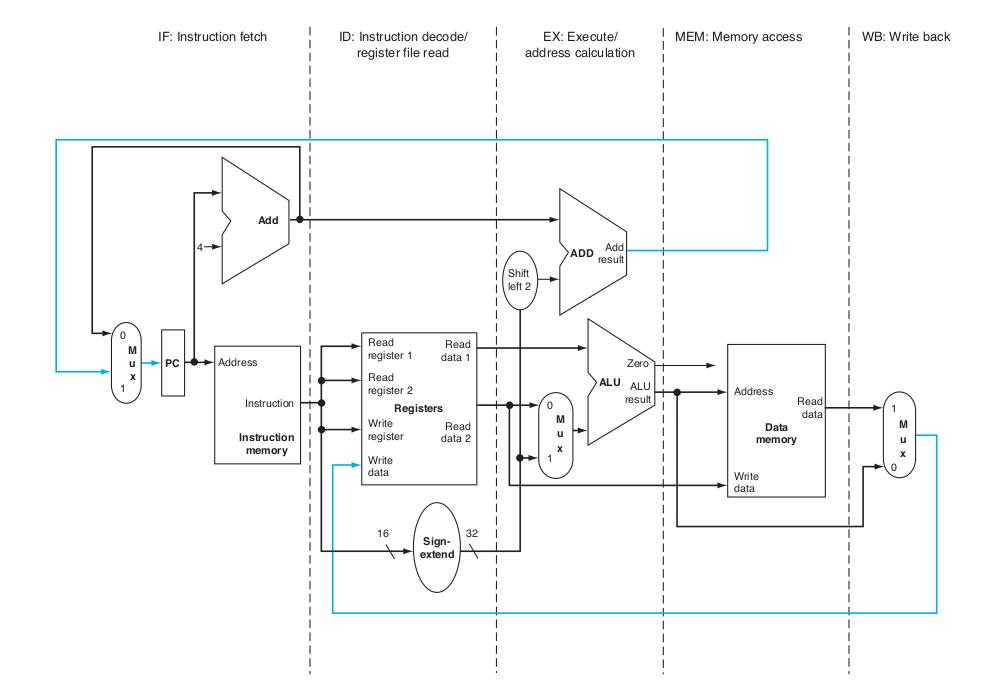
\includegraphics[width=1.1\textwidth]{imagenes/esquema_pipeline.jpeg}
\caption{Pipeline de cinco etapas: Diagrama \cite{patterson}}
\label{fig:pipeline}
\end{figure}

\subsection{\textit{IF o Instruction Fetch}}
Es la primer etapa del pipeline. Se busca la siguiente instrucción a ejecutar en la memoria de programa. En ésta etapa se ubica el contador de programa o \textit{Program Counter}, mejor conocido como PC, el cual es un registro que contiene la dirección actual en la memoria de programa en la que se encuentra el programa en ejecución. La siguiente instrucción a ejecutar antes del ciclo es PC + WORD\_SIZE (4 para un procesador de 32bits), en caso que no haya un salto. Para mejor claridad, los pasos que ocurren en el ciclo son:

\begin{enumerate}
    \item Se calcula el nuevo valor de PC. Para eso existe un multiplexor a la entrada del PC que toma el valor desde dos fuentes. La primera es el módulo sumador, que simplemente devuelve la siguiente instrucción, y la otra fuente es una dirección arbitraria que viene desde la etapa de ejecución, producto de una instrucción de salto, condicional o absoluta.
    \item Con el valor del PC se accede a la memoria de programa, se obtiene el valor en dicha dirección, y se entrega a la siguiente etapa.
\end{enumerate}

\subsection{\textit{ID o Instruction Decode}}
Etapa en donde se decodifica la instrucción y se cargan los registros correspondientes. Aqui tiene lugar el File Register, el módulo encargado de contener los 32 registros de 32bits del MIPS. Cada instrucción se transforma en sus correspondientes señales en la Unidad de Control, el cual comanda todo el procesador, según que instrucción se esté ejecutando.

\subsection{\textit{EX o Excecute}}
Unidad que ejecuta la instrucción, osea, que efectua el cálculo aritmético, lógico, o de resolución de dirección de offset. Vemos que una entrada de la ALU de propósito general puede ser un valor inmediato, con el signo extendido, o un registro, mientras que la otra entrada es siempre un registro. Existe otra ALU que unicamente suma, la cual cálcula nuevas direcciones para el PC, el cual le suma a este un valor inmediato, el cual corresponde al salto a efectuar.

\subsection{\textit{MEM o Memory Access}}
Unidad de lectura o escritura desde/hacia la memoria de datos. En ésta etapa se lee o escribe un dato de la memoria de acuerdo a la instrucción ejecutada. Si la instrucción no es de acceso a memoria, se hace un bypass de ésta etapa hacia la siguiente.

\subsection{\textit{WB o Write back}}
Escritura de resultados en los registros. Los registros pueden ser escritos desde un dato en memoria, si la instrucción era de acceso a memoria, o desde la ALU si no lo eran. Se llama Write Back porque escriben sobre una etapa anterior del pipeline.

\section{Pipeline de cinco etapas: Problema completo y solución}

El primer pipeline presentado, es simple, funciona y expone correctamente la teória básica de la segmentación en el diseño de un procesador, lo cual es necesario para el marco de este trabajo, pero presenta problemas muy grandes, que de no ser solucionados, prácticamente elimina las ventajas del pipeline debido a su ineficiencia a la hora de enfrentar ciertos casos comunes.

El presente trabajo no planea ser una explicación teórica de todas las técnicas utilizadas y los problemas resueltos, por eso se irá al grano de la implementación completa, pero dejando al lector la posibilidad de consultar la bibliografía en el caso de ser necesario. Sin embargo, se explicará brevemente el motivo de cada uno de los elementos incluidos en el mismo y luego se discutirá la implementación desarrollada. No se incluirán en el informe todos los detalles implementativos, dado que estos pueden consultarse en el código del proyecto anexo, pero se mostraran ejemplos variados y detalles a tener en cuenta.

Un esquema aproximado de la implementación completa del pipeline es el de la (Figura~\ref{fig:pipelinecompleto}).

\begin{figure}[ht]
\centering
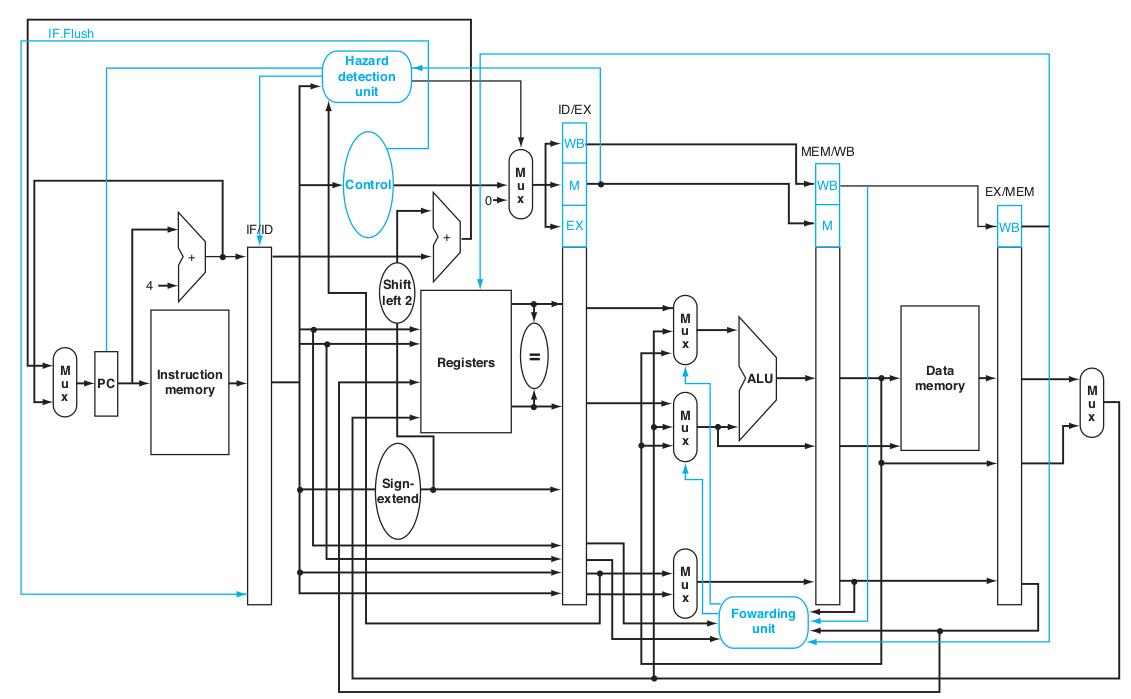
\includegraphics[width=1\textwidth]{imagenes/esquema_pipeline_completo.jpeg}
\caption{Pipeline de cinco etapas completo \cite{patterson}}
\label{fig:pipelinecompleto}
\end{figure}

Podemos ver como se agregan diferentes unidades y complejidad que resuelven problemas determinados. Los mas significativos son los latches intermedios \textit{etapa-1/etapa}, la unidad de detección de riesgos o \textit{hazard detection unit}, la unidad de control, la unidad de forwarding, y en nuestro caso, la unidad de saltos o \textit{branching unit}. A continuación se hablara de cada una de esas unidades, explicando brevemente el funcionamiento de las mismas.

\subsection{Latches intermedios}

Las etapas deben pasarse datos unas a las otras, y mas de una vez, una etapa debe obtener datos de mas de una etapa anterior a ella misma. Si una etapa deseara hacer esto, sin interbloqueo, le resultaría imposible, dado que el estado de una etapa anterior ya ha cambiado con respecto a la instrucción que le corresponde. Por este motivo se incluyen registros o latches intermedios entre cada etapa, que almacenan los datos necesarios para el flujo del pipeline. Sirven de buffer general a las señales que se deseen conservar.

Estos latches se nombran de acuerdo a las etapas que unen. Por ejemplo, el registro que une la etapa IF con la etapa ID se llama IF/ID. Veamos la implementación del \textit{latch} IF/ID:

\noindent \textit{IF\_ID.v}
\begin{lstlisting}[language=verilog]
module IF_ID
#(
    parameter PC_BITS          = `PC_BITS,
    parameter INSTRUCTION_BITS = `INSTRUCTION_BITS
)
(
    input clk,
    input rst,
    input enable,
    input flush,
    input                                  i_if_id_write,
    input wire [PC_BITS - 1 : 0]           i_PCNext,
    input wire [INSTRUCTION_BITS - 1 : 0]  i_instruction,
    output reg [PC_BITS - 1 : 0]           o_PCNext,
    output reg [INSTRUCTION_BITS - 1 : 0]  o_instruction
);

    always@(posedge clk) begin
        if (~rst) begin
            o_PCNext <= 0;
            o_instruction <= 0;
        end
        else begin
            if(enable) begin
                if (flush) begin
                    o_PCNext <= 0;
                    o_instruction <= 0;
                end
                else if (i_if_id_write) begin
                    o_PCNext <= i_PCNext;
                    o_instruction <= i_instruction;
                end
            end
        end
    end

endmodule

\end{lstlisting}

Todos los \textit{latches} simplemente pone a su salida los registros de entrada luego de un ciclo de clock, si esta el \textit{write enable} activado. Tambien tienen capacidad de flush

\subsection{Hazard detection unit}

Para explicar qué hace esta unidad tenemos que analizar algunos conceptos teóricos. El más importante es el de \textit{hazard}, o riesgo. Un riesgo ocurre cuando una instrucción no se puede ejecutar inmediatamente despues que otra, debido a dependencias no resueltas que existen entre ambas. Existen varios tipos de riesgos, los cuales se explicaran a continuacion:

\subsubsection{Tipos de riesgos}

\begin{enumerate}
    \item \textbf{Riesgo estructural:} Este tipo de riesgo ocurre cuando el hardware no puede ejecutar la combinacion de instrucciones que tenemos en el pipeline en un ciclo de reloj. Por ejemplo en el caso que en dos etapas diferentes se utilice un mismo recurso de hardware. Estos casos no se presentan a menudo dado que la idea primordial del MIPS es que sea segmentado y se eviten los riesgos estructurales.
    \item \textbf{Riesgo de datos:} Ocurren cuando el pipeline debe ser detenido porque una etapa debe esperar a que otra etapa termine. \\

    Por ejemplo:
    \begin{lstlisting}
    sub   $2, $1,$3
    and   $12,$2,$5
    \end{lstlisting}

    La instruccion \textit{sub} no escribe su resultado hasta la quinta etapa (WB), entonces se deberia detener el pipeline durante tres ciclos hasta que termine, para luego ejecutar la \textit{and}, dañando severamente la performance. El compilador podria mitigar mucho este problema, pero ocurre demasiado a menudo y no se puede confiar en que lo resuelva siempre. Existen dos maneras de solucionar este problema, haciendo una parada del pipeline (poco eficiente) o implementando una \textit{forwarding unit}. Ésta es la técnica utilizada en este trabajo, de la cual se hablara más adelante.
    \item \textbf{Riesgo de control:} Se basa en la necesidad de tomar una desicion sin conocer el resultado de una instruccion que esta ejecutandose. Estas instrucciones, mas especificamente, son las de \textif{branching} o de salto. Cuando entra una instruccion de salto al pipeline, dependiendo de si ese salto es tomado o no, la etapa IF debe cargar nuevas instrucciones de un lado de la memoria u otro. Para resolver este problema se usan predictores de salto, que tratan de adivinar cual sera el resultado del salto. En el caso de adivinar correctamente, la performance no se ve afectada, si no es asi, deben desecharse las instrucciones que habia en el pipeline hasta ese momento, y comenzar a cargar las nuevas. Los tipos de predictores no seran explicados aqui, salvo el elegido por los autores, el cual es llamado \textit{branch not taken}. este tipo de predictor siempre supone que el branch no es tomado. Es menos eficiente que soluciones más complejas, pero es simple de implementar y en bajo en consumo de recursos de hardware.
\end{enumerate}

\noindent En vista de los tipos de riesgos que hay, y sus necesidades, nuestra \textit{hazard detection unit} se ubicará en la etapa de ID, y solo contendrá lógica para la detección y salida de control de los riesgos de datos:

\noindent \textit{HazardDetector.v}
\begin{lstlisting}[language=verilog]
module HazardDetector
#(
    parameter INSTRUCTION_BITS = `INSTRUCTION_BITS,
    parameter REG_ADDRS_BITS   = `REG_ADDRS_BITS
)
(
    input wire [REG_ADDRS_BITS - 1 : 0] i_instruction_rs,
    input wire [REG_ADDRS_BITS - 1 : 0] i_instruction_rt,
    input wire [REG_ADDRS_BITS - 1 : 0] i_id_ex_rt,
    input wire                          i_id_ex_MemRead,
    output reg                          o_PCWrite,
    output reg                          o_if_id_write,
    output reg                          o_control_mux
);

    //control_mux = 0 when we want to set all control lines to 0 and
    //control mux = 1 when we want all control lines from the control unit
    always@* begin
        if  (
                i_id_ex_MemRead &&
                (
                    (i_id_ex_rt == i_instruction_rs) ||
                    (i_id_ex_rt == i_instruction_rt)
                )
            )
        begin
            o_PCWrite     = 0;
            o_if_id_write = 0;
            o_control_mux = 0;
        end
        else begin
            o_PCWrite     = 1;
            o_if_id_write = 1;
            o_control_mux = 1;
        end
    end
endmodule

\end{lstlisting}

\noindent Se evalúan las situaciones peligrosas:
\begin{itemize}
  \item Si la instrucción anterior quiere leer (\textit{i\_id\_ex\_MemRead}) y:
  \begin{itemize}
    \item Si el registro RT de la instruccion anterior (\textit{i\_id\_ex\_rt}) es igual al RS de la actual (\textit{i\_instruction\_rs}) o...
    \item Si el registro RT de la instruccion anterior (\textit{i\_id\_ex\_rt}) es igual al RT de la actual (\textit{i\_instruction\_rt}).
  \end{itemize}
\end{itemize}

\noindent Si se cumple alguno de esos casos el riesgo fue detectado y se toman las medidas correspondientes.

\subsection{Control Unit}

Para explicar la Unidad de Control, debemos abordar un enfoque de más pequeño a más grande. Existe una Unidad de Control principal y una Unidad de Control de ALU (no representada en el diagrama general) pero sobre la cual se hablará a continuación. Para tener un mejor entendimiento del tema, es bueno entender como se componen binariamente las instrucciones del set de instrucciones MIPS de 32 bits, según el tipo de instrucción que sean. La (Figura~\ref{fig:instrucciones}) detalla esta estructura. Prestar atencion al campo \textit{op}, \textit{shamt}, y \textit{funct}, dado que son campos de los que no se ha hablado hasta ahora.

\begin{figure}[ht]
\centering
\hspace*{-1cm}
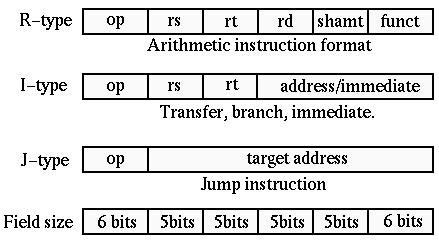
\includegraphics[width=.5\textwidth]{imagenes/estructura_instrucciones.jpeg}
\caption{Estructura binaria de cada tipo de instruccion}
\label{fig:instrucciones}
\end{figure}

\subsubsection{ALU Control}

Dependiendo del tipo de instrucción a ejecutar, la ALU deberá efectuar una de ciertas operaciones definidas. Éstas operaciones se seleccionan mediante lineas de control de la ALU. El (Cuadro~\ref{tab:alucontrol}) las define, según el standard MIPS.

\begin{table}[!ht]
\centering
\caption{Combinación de entradas de control de ALU y funciones a las que mapean}
\label{tab:alucontrol}
\smallskip
\begin{tabular}{l c c}
\hline
Control ALU & Función \\[0.5ex]
\hline
&&\\[-2ex]
0000 & AND \\[0.5ex]
\hline
&&\\[-2ex]
0001 & OR\\[0.5ex]
\hline
&&\\[-2ex]
0010 & add\\[0.5ex]
\hline
&&\\[-2ex]
0110 & substract\\[0.5ex]
\hline
&&\\[-2ex]
0111 & set on less than\\[0.5ex]
\hline
&&\\[-2ex]
1100 & NOR\\[0.5ex]
\hline
\end{tabular}
\end{table}

Que familias de instrucciones mapeen a las mismas operaciones de ALU nos permite generar otro nivel de abstracción para el control de la ALU y las instrucciones a ejecutar. Con una señal de dos bits llamada \textit{ALUOp} podemos mapear a dichas operaciones. La tabla (Cuadro~\ref{tab:alucontrolops}) muestra este nuevo concepto. También se intruduce el concepto de Funct Field, el cual es un campo de cada instrucción de MIPS el cual, junto con el Opcode, definen la instrucción a ejecutar.

\begin{table}[!ht]
\centering
\caption{Mapeo \textit{ALUOps} a Funct field y entradas de control de ALU}
\label{tab:alucontrolops}
\smallskip
\begin{tabular}{l c c c c c}
\hline
Opcode & ALUOp & Operación & Funct field & Operación ALU & Control ALU\\[0.5ex]
\hline
&&\\[-2ex]
LW & 00 & load word & XXXXXX & add & 0010\\[0.5ex]
\hline
&&\\[-2ex]
SW & 00 & store word & XXXXXX & add & 0010\\[0.5ex]
\hline
&&\\[-2ex]
Branch equal & 01 & branch equal & XXXXXX & substract & 0110\\[0.5ex]
\hline
&&\\[-2ex]
Tipo R & 10 & add & 100000 & add & 0010\\[0.5ex]
\hline
&&\\[-2ex]
Tipo R & 10 & substract & 100010 & substract & 0110\\[0.5ex]
\hline
&&\\[-2ex]
Tipo R & 10 & AND & 100100 & AND & 0000\\[0.5ex]
\hline
&&\\[-2ex]
Tipo R & 10 & OR & 100101 & OR & 0001\\[0.5ex]
\hline
&&\\[-2ex]
Tipo R & 10 & set on less than & 101010 & set on less than & 0111\\[0.5ex]
\hline
\end{tabular}
\end{table}

La implementación es extensa debido a las definiciones requeridas, por eso se omiten algunas partes del código:

\noindent \textit{ALUControl.v}
\begin{lstlisting}[language=verilog]
module ALUControl
(
    input wire [3 : 0] i_ALUOp,
    input wire [5 : 0] i_funct,

    output reg [3 : 0] o_operation
);
    localparam ALU_ADD  = 'b0000;
    localparam ALU_SUB  = 'b0001;
    // ... resto de AluOP
    localparam FUNCT_ADD  = 'b100000;
    localparam FUNCT_ADDU = 'b100001;
    // ... resto de Functs
    localparam INMED_ADD  = 'b000;
    localparam INMED_AND  = 'b100;
    // ... resto de AluOp

    always@* begin
        if (i_ALUOp == 'b0000) begin
            case (i_funct)
                FUNCT_ADD:  o_operation = ALU_ADD;
                FUNCT_ADDU: o_operation = ALU_ADD;
                // ... resto del mapeo
                default:    o_operation = 0;
            endcase
        end

        else if (i_ALUOp == 'b0001) begin
            o_operation = ALU_ADD;
        end

        else if (i_ALUOp[3] == 1) begin
            case (i_ALUOp[2:0])
                INMED_ADD: o_operation = ALU_ADD;
                INMED_AND: o_operation = ALU_AND;
                // ... resto del mapeo
                default:   o_operation = 0;
            endcase
        end
        else o_operation = 0;
   end
endmodule
\end{lstlisting}

\noindent Se ve como se hace un mapeo, teniendo en cuenta las diferentes variaciones que hay en el set de instrucciones, ALUOps, Functs y controles de la ALU.

\subsubsection{Main Control Unit}

Ahora que ya definimos los controles de la ALU, y como interpretarlos a partir de los bits de la instruccion, debemos definir como se controlan todas las otras partes del datapath. En la (Figura~\ref{fig:controlsig}) se observan en celeste, cuales son las principales señales de control de los diferentes elementos del pipeline.

\begin{figure}[ht]
\centering
\hspace*{-1cm}
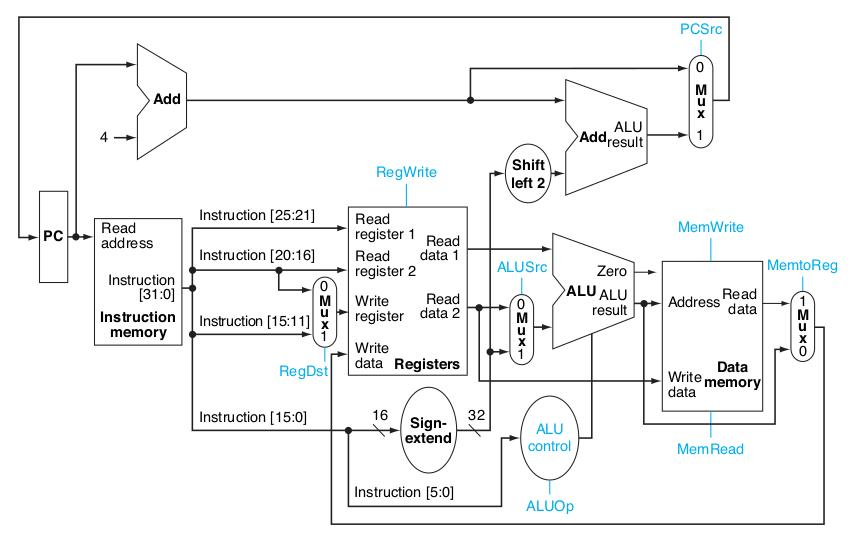
\includegraphics[width=1.1\textwidth]{imagenes/controlsig.jpeg}
\caption{Señales de control del pipeline \cite{patterson}}
\label{fig:controlsig}
\end{figure}

Éstas siete señales tienen diferentes efectos, los cuales se explican en el (Cuadro~\ref{tab:controlsigcuadro}).

\begin{table}[!ht][H]
\centering
\caption{Señales de control de la \textit{Main Control Unit}}
\label{tab:controlsigcuadro}
\smallskip
\begin{tabular}{l c c}
\hline
Nombre de la señal & Efecto en bajo & Efecto en alto\\[0.5ex]
\hline
&&\\[-2ex]
RegDst & El número del registro de destino & Idem RD \\& viene del campo RT\\[0.5ex]
\hline
&&\\[-2ex]
RegWrite & Nada & El registro en la entrada \\&&es escrito con el valor del dato \\[0.5ex]
\hline
&&\\[-2ex]
ALUSrc & El segundo operando & Idem del extensor de signo \\&de la ALU viene de la segunda \\&salida de los registros \\[0.5ex]
\hline
&&\\[-2ex]
PCSrc & El PC es reemplazado con & Idem con el objetivo del salto \\&la salida del sumador PC+4  \\[0.5ex]
\hline
&&\\[-2ex]
MemRead & Nada & Se lee la memoria \\&&a partir de sus entradas \\[0.5ex]
\hline
&&\\[-2ex]
MemWrite & Nada & Se escribe la memoria \\&& a partir de sus entradas \\[0.5ex]
\hline
&&\\[-2ex]
MemToReg & El valor entregado & Idem memoria de datos\\& a los datos de escritura del registro \\&vienen de la ALU \\[0.5ex]
\hline
\end{tabular}
\end{table}

Habiendo entendido cuales son las entradas y salidas que gobiernan el módulo de control, veremos la implementación del mismo. Tener en cuenta que tambien se producen truncaciones en el código (no sin comentarlas y no sin que ya haya sido explicada como completarlo) para brevedad.

\noindent \textit{Control.v}
\begin{lstlisting}[language=verilog]
`include "constants.vh"

module Control
#(
    parameter OPCODE_BITS = `OPCODE_BITS
)
(
    input wire [OPCODE_BITS - 1 : 0] i_opcode,
    input wire [5: 0]                i_funct,
    input wire                       i_control_mux,
    output reg                       o_RegDst,
    output reg                       o_RegWrite,
    output reg                       o_MemRead,
    output reg                       o_MemWrite,
    output reg                       o_MemtoReg,
    output reg [3:0]                 o_ALUOp,
    output reg                       o_ALUSrc,
    output reg                       o_Shamt,
    output reg [2:0]                 o_ls_filter_op
);

    localparam LW      = 'b100;
    localparam SW      = 'b101;
    localparam INMED   = 'b001;
    localparam OTHER   = 'b000;

    always@* begin
        o_ls_filter_op  = i_opcode[2:0];

        if (i_control_mux) begin
            case (i_opcode[5:3])
                LW: begin
                    // El primero se expone para claridad
                    // Los otros casos se colapsan
                    o_RegDst   = 0;
                    o_RegWrite = 1;
                    o_MemRead  = 1;
                    o_MemWrite = 0;
                    o_MemtoReg = 1;
                    o_ALUOp    = 'b0001;
                    o_ALUSrc   = 1;
                    o_Shamt    = 0;
                end

                SW: begin
                    // Caso de instruccion SW
                end

                INMED: begin
                    // Caso de instruccion inmediata
                end

                OTHER: begin
                    if (i_opcode[2]) begin
                        // Caso de branch
                    end

                    else if (i_opcode[1]) begin
                      //Caso de J-JAL
                    end

                    else if (i_opcode == 0) begin
                        if (i_funct[5:1] == 'b00100) begin
                           // Caso de JR-JRAL
                        end

                        else begin
                          // Caso de RTYPE
                        end
                    end
                    else begin
                        // Caso ninguna instruccion. Stall
                    end
                end

                default: begin
                    // Caso ninguna instruccion. Stall
                end
            endcase
        end

        else begin
            // Caso ninguna instruccion. Stall
        end

    end

endmodule

\end{lstlisting}

\subsection{Forwarding Unit}

Como se mencionó anteriormente, existen dos maneras de lidiar con los riesgos de datos. Parar el pipeline hasta que se resuelvan las dependencias al escribirse nuevamente en la etapa WB, o implementar una \textit{forwarding unit}. Lo que hace este modulo es detectar si alguna instrucción que se encuentre en el pipeline va a necesitar un dato que este ya esté en EX o WB, y lo envía directamente, sin necesidad de que este haya sido escrito todavia en un registro. Nótese que existe el caso donde el dato requerido por la instrucción siguiente viene a partir de un load. Los load se procesan en la etapa siguiente a EX, en MEM, lo que pone dos etapas de distancia entre la instrucción que requiere el dato, y el dato en sí. Esto obliga a que haya una parada de un ciclo, hasta que se resuelve el load, y pueda ser forwardeado a la etapa de ejecución.

\noindent \textit{ForwardingUnit.v}
\begin{lstlisting}
module FowardingUnit
#(
    parameter REG_ADDRS_BITS = `REG_ADDRS_BITS
)
(
    input wire i_ex_mem_RegWrite,
    input wire i_mem_wb_RegWrite,
    input wire [REG_ADDRS_BITS - 1 : 0] i_id_ex_rs,
    input wire [REG_ADDRS_BITS - 1 : 0] i_id_ex_rt,
    input wire [REG_ADDRS_BITS - 1 : 0] i_ex_mem_rd,
    input wire [REG_ADDRS_BITS - 1 : 0] i_mem_wb_rd,

    output reg [1:0] o_foward_A,
    output reg [1:0] o_foward_B
);

    reg mem_foward_a;
    reg mem_foward_b;
    reg wb_foward_a;
    reg wb_foward_b;

    always@* begin

        mem_foward_a = i_ex_mem_RegWrite && (i_ex_mem_rd != 0) &&
                       (i_ex_mem_rd == i_id_ex_rs);
        mem_foward_b = i_ex_mem_RegWrite && (i_ex_mem_rd != 0) &&
                       (i_ex_mem_rd == i_id_ex_rt);
        wb_foward_a  = i_mem_wb_RegWrite && (i_mem_wb_rd != 0) &&
                       (i_mem_wb_rd == i_id_ex_rs);
        wb_foward_b  = i_mem_wb_RegWrite && (i_mem_wb_rd != 0) &&
                       (i_mem_wb_rd == i_id_ex_rt);

        if (mem_foward_a)     o_foward_A = 'b10;
        else if (wb_foward_a) o_foward_A = 'b01;
        else                  o_foward_A = 'b00;

        if (mem_foward_b)     o_foward_B = 'b10;
        else if (wb_foward_b) o_foward_B = 'b01;
        else                  o_foward_B = 'b00;
    end
endmodule
\end{lstlisting}

\noindent Como se explicó el módulo analiza las necesidades de las etapas anteriores en busqueda de una dependencia que puede ser cumplida inmediatamente. De ser así, envía ese dato a la entrada de la ALU correspondiente.

\subsection{Branching Unit}

Esta unidad es una solución propia para resolver el control de saltos. Interpreta los \textit{opcodes} de cada instrucción y controla las señales correspondientes. Esto alivia trabajo de la Unidad de Control. Además contiene la lógica del predictor de saltos. Decide si se va a interpretar como \textit{taken} o \textit{not taken}.

\noindent \textit{BranchUnit.v}
\begin{lstlisting}[language=verilog]
`include "constants.vh"

module BranchUnit
#(
    parameter OPCODE_BITS = `OPCODE_BITS,
    parameter PROC_BITS   = `PROC_BITS,
    parameter PC_BITS     = `PC_BITS,
    parameter FUNCT_BITS  = `FUNCT_BITS
)
(
    input wire                       i_branch_enable,
    input wire [OPCODE_BITS - 1 : 0] i_opcode,
    input wire [FUNCT_BITS - 1 : 0]  i_funct,
    input wire [PC_BITS - 1 : 0]     i_pc_next,
    input wire [PROC_BITS - 1 : 0]   i_immediate,
    input wire [PROC_BITS - 1 : 0]   i_jump_address,
    input wire [PROC_BITS - 1 : 0]   i_data_rs,
    input wire [PROC_BITS - 1 : 0]   i_data_rt,

    output reg o_taken,
    output reg o_pc_to_reg,
    output reg [PC_BITS - 1 : 0] o_jump_address,
    output reg [PC_BITS - 1 : 0] o_pc_return,
    output reg o_pc_reg_sel

);

    localparam BEQ     = 'b000100;
    localparam BNE     = 'b000101;
    localparam J       = 'b000010;
    localparam JAL     = 'b000011;
    localparam JR_JALR = 'b000000;

    always@* begin
        o_pc_return = i_pc_next;
        if (i_branch_enable) begin
            case (i_opcode)
                BEQ: begin
                    o_taken = i_data_rs == i_data_rt;
                    o_pc_to_reg = 0;
                    o_jump_address = (i_pc_next + i_immediate);
                    o_pc_reg_sel = 0;
                end
                BNE: begin
                    o_taken = i_data_rs != i_data_rt;
                    o_pc_to_reg = 0;
                    o_jump_address = (i_pc_next + i_immediate);
                    o_pc_reg_sel = 0;
                end
                J: begin
                    o_taken = 1;
                    o_pc_to_reg = 0;
                    o_jump_address = i_jump_address;
                    o_pc_reg_sel = 0;
                end
                JAL: begin
                    o_taken = 1;
                    o_pc_to_reg = 1;
                    o_jump_address = i_jump_address;
                    o_pc_reg_sel = 1;
                end
                JR_JALR: begin
                    //JR
                    if (i_funct == 'b001000) begin
                        o_taken = 1;
                        o_pc_to_reg = 0;
                        o_jump_address = i_data_rs;
                        o_pc_reg_sel = 0;
                    end
                    //JALR
                    else if (i_funct == 'b001001) begin
                        o_taken = 1;
                        o_pc_to_reg = 1;
                        o_jump_address = i_data_rs;
                        o_pc_reg_sel = 0;
                    end
                    //NO JUMP
                    else begin
                        o_taken = 0;
                        o_pc_to_reg = 0;
                        o_jump_address = 0;
                        o_pc_reg_sel = 0;
                    end
                end
                //NO JUMP
                default: begin
                    o_taken = 0;
                    o_pc_to_reg = 0;
                    o_jump_address = 0;
                    o_pc_reg_sel = 0;

                end
            endcase
        end
        else begin
            o_taken = 0;
            o_pc_to_reg = 0;
            o_jump_address = 0;
            o_pc_reg_sel = 0;
        end
    end
endmodule
\end{lstlisting}

\section{Debug Unit}

Como se comento anteriormente, la Debug Unit es fundamental para el analísis y utilización del pipeline sintetizado. Sin este, es un proyecto inerte e inutilizable.

Dicha unidad se conecta, en el módulo principal, a las lineas del Datapath que existen para este propósito. El Datapath debió ser modificado de manera importante para la inclusión de ésta unidad, dado que los datos que se desean extraer de la misma son de variada indole y procedencia.

La Debug Unit esta modelada como una máquina de estados finita, cuyo diagrama se presenta en el (Diagrama~\ref{fig:fsm}).

\begin{center}
\begin{tikzpicture}[scale=0.2]
\tikzstyle{every node}+=[inner sep=0pt]
\draw [black] (43.7,-23.8) circle (3);
\draw (43.7,-23.8) node {$IDLE$};
\draw [black] (64.8,-10.3) circle (3);
\draw (64.8,-10.3) node {$START\_LOAD$};
\draw [black] (22.3,-48.3) circle (3);
\draw (22.3,-48.3) node {$START\_RUN$};
\draw [black] (12.4,-14.5) circle (3);
\draw (12.4,-14.5) node {$START\_STEP$};
\draw [black] (67.4,-34.6) circle (3);
\draw (67.4,-34.6) node {$WAIT\_LOAD$};
\draw [black] (42.4,-45.9) circle (3);
\draw (42.4,-45.9) node {$WAIT\_RUN$};
\draw [black] (11.8,-29.1) circle (3);
\draw (11.8,-29.1) node {$WAIT\_STEP$};
\draw [black] (44.467,-20.904) arc (160.09544:85.12763:16.955);
\fill [black] (61.85,-9.78) -- (61.09,-9.22) -- (61.01,-10.21);
\draw (41.55,-11.89) node [above] {$i\_rx\_data=LOAD\_INS$};
\draw [black] (41.73,-26.06) -- (24.27,-46.04);
\fill [black] (24.27,-46.04) -- (25.18,-45.77) -- (24.42,-45.11);
\draw (32.46,-34.6) node [left] {$i\_rx\_data=RUN\_STEP$};
\draw [black] (15.375,-14.119) arc (94.97419:51.92985:37.025);
\fill [black] (15.37,-14.12) -- (16.22,-14.55) -- (16.13,-13.55);
\draw (34.91,-14.66) node [above] {$i\_rx\_data=RUN$};
\draw [black] (45.396,-21.34) arc (173.14616:-114.85384:2.25);
\draw (50.26,-19.31) node [right] {$else$};
\fill [black] (46.68,-23.65) -- (47.42,-24.24) -- (47.54,-23.25);
\draw [black] (66.28,-12.908) arc (26.41577:-14.20142:27.281);
\fill [black] (68.29,-31.74) -- (68.98,-31.09) -- (68.01,-30.84);
\draw [black] (46.55,-24.737) arc (70.98121:60.02164:105.143);
\fill [black] (46.55,-24.74) -- (47.14,-25.47) -- (47.47,-24.53);
\draw (62.42,-27.91) node [above] {$load\_fsm\_done$};
\draw [black] (68.171,-37.487) arc (42.69007:-245.30993:2.25);
\draw (62.15,-42.33) node [below] {$!load\_fsm\_done$};
\fill [black] (65.58,-36.97) -- (64.65,-37.14) -- (65.33,-37.88);
\draw [black] (44.313,-26.736) arc (9.45568:-16.1886:36.833);
\fill [black] (44.31,-26.74) -- (43.95,-27.61) -- (44.94,-27.44);
\draw (45.34,-34.98) node [right] {$run\_fsm\_done$};
\draw [black] (44.241,-48.254) arc (65.76829:-222.23171:2.25);
\draw (47.68,-53.57) node [below] {$!run\_fsm\_done$};
\fill [black] (41.65,-48.79) -- (40.87,-49.32) -- (41.78,-49.73);
\draw [black] (11.369,-26.132) arc (-174.44864:-190.25795:31.693);
\fill [black] (11.37,-26.13) -- (11.79,-25.29) -- (10.79,-25.38);
\draw [black] (40.841,-24.708) arc (-73.2083:-87.92531:103.058);
\fill [black] (40.84,-24.71) -- (39.93,-24.46) -- (40.22,-25.42);
\draw (30.81,-28.82) node [below] {$step\_fsm\_done$};
\draw [black] (11.536,-32.077) arc (22.67131:-265.32869:2.25);
\fill [black] (9.28,-30.7) -- (8.35,-30.55) -- (8.73,-31.47);
\draw [black] (40.568,-48.267) arc (-44.43571:-121.94619:12.815);
\fill [black] (40.57,-48.27) -- (39.65,-48.49) -- (40.37,-49.19);
\end{tikzpicture}
\caption{Diagrama de la FSM de la DebugUnit}
\label{fig:fsm}
\end{center}

\noindent Esta máquina de estados modela el comportamiento de la unidad, pero luego existen módulos que entran en acción según en que estado se encuentre la misma. Por ejemplo, enviar datos por UART, cargar un programa, ejecutar el programa, son todas tareas comandadas por la máquina de estados general. Para conocer más sobre los detalles de la implementación, consultar el código anexo.

\section{Test Benches}

\noindent Los \textif{test benches} son una parte fundamental de cada diseño en cualquier HDL. Estos componen el primer paso en la validacion del sistema, y deben ser pasados para continuar a cualquier etapa posterior. Consisten en una representación lógica de cada módulo, a la cual luego se lo ataca con señales de entrada simuladas, pensadas para contemplar la mayor cantidad de casos posibles. El resultado de la prueba es exitoso si la salída esperada se corresponde con la salída real. La suite de desarrollo que utilizamos cuenta con herramientas de simulación, muy utiles para ésta tarea.

Debe tenerse en cuenta que un \textif{test bench} exitoso no corresponde a una implementación sintetizada exitosa. Existen problemas de hardware (timing, conexiones, constraints, espacio) que no son contemplados en la simulación.

En el marco de este trabajo se generaron \textif{test benches} para cada uno de los módulos utilizados. A continuación se muestra un ejemplo de estos tests, quedando a disposición el resto en el código fuente anexo.


\noindent \textit{tb\_HazardDetector.v}
\begin{lstlisting}[language=verilog]
module tb_HazardDetector();

    reg [4:0] rs;
    reg [4:0] rt;
    reg [4:0] id_ex_rt;
    reg id_ex_MemRead;
    wire PCWrite;
    wire if_id_write;
    wire control_mux;

    initial begin
        //testing MemRead == 0
        id_ex_MemRead = 0;
        rs = 0;
        rt = 0;
        id_ex_rt = 0;

        //testing all posibilities

        //all register diferent
        #20
        id_ex_MemRead = 1;
        rs = 1;
        rt = 2;
        id_ex_rt = 3;

        //rs == id_ex_rt
        #20
        id_ex_MemRead = 1;
        rs = 10;
        rt = 2;
        id_ex_rt = 10;

        //rt == id_ex_rt
        #20
        id_ex_MemRead = 1;
        rs = 10;
        rt = 25;
        id_ex_rt = 25;

        //rs == rt == id_ex_rt
        #20
        id_ex_MemRead = 1;
        rs = 15;
        rt = 15;
        id_ex_rt = 15;

        //rs == rt == id_ex_rt and MemRead == 0
        #20
        id_ex_MemRead = 0;
        rs = 15;
        rt = 15;
        id_ex_rt = 15;
    end

    HazardDetector hazard_detector_u(
        .i_instruction_rs(rs),
        .i_instruction_rt(rt),
        .i_id_ex_rt(id_ex_rt),
        .i_id_ex_MemRead(id_ex_MemRead),
        .o_PCWrite(PCWrite),
        .o_if_id_write(if_id_write),
        .o_control_mux(control_mux)
    );
endmodule
\end{lstlisting}

Se ve a simple vista como las entradas del modulo son confeccionadas para probar cada caso de interés. En la (Figura~\ref{fig:simulacion}) vemos la salída gráfica que nos provee la herramienta de simulación para analizar los resultados obtenidos. También existen formas de incluir asserts para generar tests automatizados de los módulos y no tener que analizar las gráficas todo el tiempo, pero en el módulo mostrado en este informe no se utilizan por conveniencia.

\begin{figure}[ht]
\centering
\hspace*{-1cm}
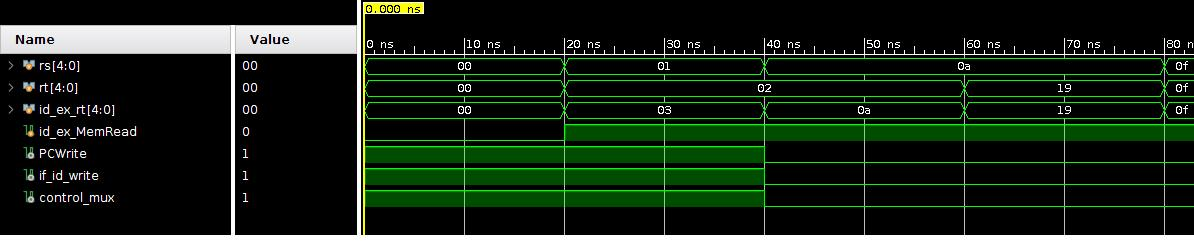
\includegraphics[width=1\textwidth]{imagenes/simulacion.jpeg}
\caption{Simulación módulo HazardDetector.v [Xilinx Vivado]}
\label{fig:simulacion}
\end{figure}

Nótese también, como en éstas simulaciones se pueden realizar cosas imposibles en módulos que planeen ser sintetizados. Por ejemplo, incluir delays de tiempo (con \textit{\#xx}) no es sintetizable en hardware.

\section{Tests sobre el modelo sintetizado}

Una vez sintetizado y cargado en el embebido FPGA, es necesario comprobar el correcto funcionamiento del pipeline. Una buena forma de realizar esto es automatizar la tarea utilizando los datos obtenidos de la Debug Unit mediante UART. Pudiendo cargar un programa, y obtener resultados, es totalmente posible generar un pequeño programa controlador y comparador. Creando un script en Python y utilizando una librería de test genéricos llamada \textit{pytest} se creó esta utilidad.

Los resultados de la herramienta son de muy simple lectura, como se puede ver en la (Figura~\ref{fig:test}), lo que facilita la tarea del desarrollador a la hora de aplicar cambios, y comprobar que estos no afecten el comportamiento del procesador.

\begin{figure}[ht]
\centering
\hspace*{-1cm}
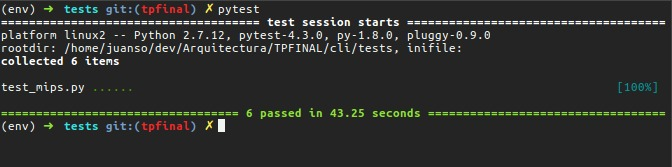
\includegraphics[width=0.95\textwidth]{imagenes/test.jpeg}
\caption{Tests automatizados sobre el hardware sintetizado}
\label{fig:test}
\end{figure}

\section{Ensamblador}

Crear programas en código máquina es una tarea muy engorrosa, dado el manejo de bits que esto conlleva. Por ésto es que existen abstracciones que van de menor a mayor en nivel, siendo el lenguaje ensamblador la siguiente en la escala a partir del lenguaje de máquina. El lenguaje ensamblador consiste en la resolución de los símbolos mnemonicos de las instrucciones y los operandos de las mismas a una línea de lenguaje máquina. En la (Figura~\ref{fig:asm}) vemos como luce una sección de código en ensamblador, y como se traduce a lenguaje máquina.
\\
\begin{figure}[ht]
\centering

\textit{Assembler:}
\begin{lstlisting}
                        addi   $a0,   $a0,   -1
                        addi   $a1,   $zero,   1
\end{lstlisting}
\textit{Lenguaje Máquina:}
\begin{lstlisting}
                        2084ffff
                        20050001
\end{lstlisting}
\caption{Paso de ensamblador a lenguaje máquina}
\label{fig:asm}
\end{figure}

Para resolver esta tarea se generó, también con el lenguaje Python, una utilidad ensambladora básica. Hay herramientas existentes muchos más poderosas para ésta tarea, pero para este trabajo se pedía que la misma fuera generada en su marco. La implementación también se encuentra anexa en el código fuente del trabajo.

\section{Interfaz Gráfica}
Con los elementos presentados hasta el momento ya se cuenta con una implementación totalmente funcional de un pipeline de MIPS para la cual es posible debuggear y desarrollar. Para facilitar este proceso se decidió mejorar la experiencia del usuario en la parte del debugging. En una primer versión, los datos del estado interno se mostraban por terminal. Esta solución parece ineficiente desde el punto de vista del usuario, dado el poco atractivo grafico, y la dificultad de leer texto tan condensado.

Por esto se decidió crear una aplicación WEB, que soporte la misma funcionalidad que la Debug Unit y sirva de interfaz para la misma. Las herramientas utilizadas fueron de nuevo Python, agregando Flask para el desarrollo web. En la (Figura~\ref{fig:interfaz}) se puede ver el aspecto de dicha interfaz, en pleno proceso de debugging paso a paso sobre un programa.

\begin{figure}[ht]
\centering
\hspace*{-1cm}
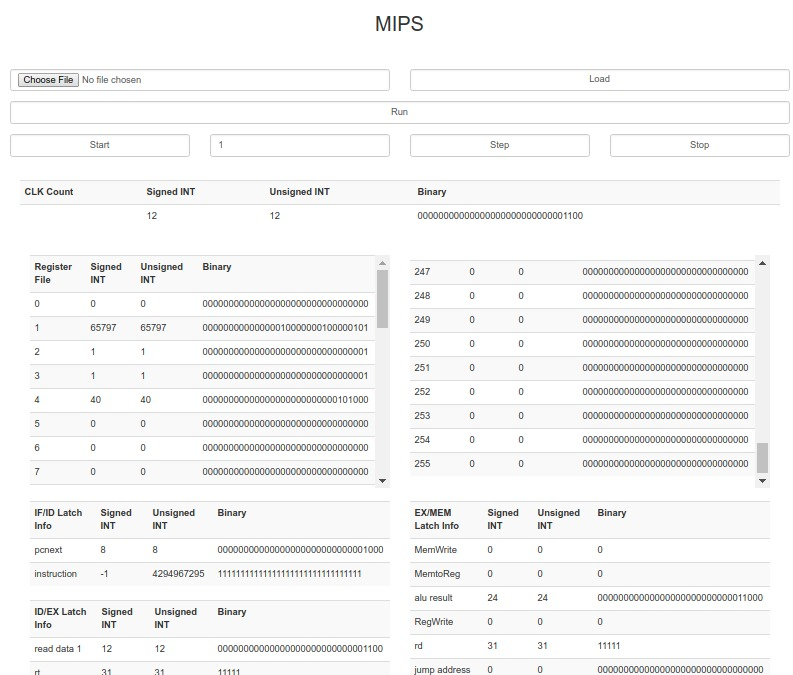
\includegraphics[width=1\textwidth]{imagenes/interfaz.jpeg}
\caption{Interfaz gráfica WEB: Debugging}
\label{fig:interfaz}
\end{figure}

\section{Consideraciones finales}

Este trabajo reúne los conocimientos básicos de la arquitectura de computadoras y su resolución es muy útil para su aprendizaje. Es un desafío bastante grande encarar un proyecto tan complejo, pero con ayuda de la bibliografía de referencia, y tiempo y dedicación puede lograrse. Esto asienta las bases de un buen conocimiento en el area de procesadores de propósito general y de prototipado de hardware, las cuales son fundamentales en la formación de un Ingeniero en Computación.

\bibliographystyle{sbc}
\bibliography{sbc-template}

\end{document}
